\documentclass{article} % For LaTeX2e
\usepackage{iclr2024_conference,times}

\usepackage[utf8]{inputenc} % allow utf-8 input
\usepackage[T1]{fontenc}    % use 8-bit T1 fonts
\usepackage{hyperref}       % hyperlinks
\usepackage{url}            % simple URL typesetting
\usepackage{booktabs}       % professional-quality tables
\usepackage{amsfonts}       % blackboard math symbols
\usepackage{nicefrac}       % compact symbols for 1/2, etc.
\usepackage{microtype}      % microtypography
\usepackage{titletoc}

\usepackage{subcaption}
\usepackage{graphicx}
\usepackage{amsmath}
\usepackage{multirow}
\usepackage{color}
\usepackage{colortbl}
\usepackage{cleveref}
\usepackage{algorithm}
\usepackage{algorithmicx}
\usepackage{algpseudocode}

\DeclareMathOperator*{\argmin}{arg\,min}
\DeclareMathOperator*{\argmax}{arg\,max}

\graphicspath{{../}} % To reference your generated figures, see below.
\begin{filecontents}{references.bib}
@inproceedings{vaswani2017attention,
  title={Attention is all you need},
  author={Vaswani, Ashish and Shazeer, Noam and Parmar, Niki and Uszkoreit, Jakob and Jones, Llion and Gomez, Aidan N and Kaiser, {\L}ukasz and Polosukhin, Illia},
  booktitle={Advances in neural information processing systems},
  pages={5998--6008},
  year={2017}
}

@Article{Igo2006AGM,
 author = {S. Igo},
 booktitle = {Journal of the History of the Behavioral Sciences},
 journal = {Journal of the history of the behavioral sciences},
 pages = {
          109-34
        },
 title = {"A gold mine and a tool for democracy": George Gallup, Elmo Roper, and the business of scientific polling, 1935-1955.},
 volume = {42 2},
 year = {2006}
}


@Article{Scharr'e2024EuclidPX,
 author = {Euclid Collaboration L. Scharr'e and M. Hirschmann and G. Lucia and S. Charlot and F. Fontanot and M. Spinelli and L. Xie and A. Feltre and V. Allevato and A. Plat and M. Bremer and S. Fotopoulou and L. Gabarra and B. Granett and Michele Moresco and C. Scarlata and L. Pozzetti and L. Spinoglio and M. Talia and G. Zamorani and B. Altieri and A. Amara and S. Andreon and N. Auricchio and M. Baldi and S. Bardelli and D. Bonino and E. Branchini and M. Brescia and J. Brinchmann and S. Camera and V. Capobianco and C. Carbone and J. Carretero and S. Casas and F. Castander and M. Castellano and S. Cavuoti and A. Cimatti and G. Congedo and C. Conselice and L. Conversi and Y. Copin and L. Corcione and F. Courbin and H. Courtois and A. D. Silva and H. Degaudenzi and J. Dinis and M. Douspis and F. Dubath and X. Dupac and S. Dusini and M. Farina and S. Farrens and S. Ferriol and M. Frailis and E. Franceschi and S. Galeotta and B. Garilli and B. Gillis and C. Giocoli and A. Grazian and F. Grupp and L. Guzzo and S. Haugan and W. Holmes and I. Hook and F. Hormuth and A. Hornstrup and K. Jahnke and E. Keihanen and S. Kermiche and A. Kiessling and T. Kitching and B. Kubik and M. Kummel and M. Kunz and H. Kurki-Suonio and S. Ligori and P. Lilje and V. Lindholm and I. Lloro and D. Maino and E. Maiorano and O. Mansutti and O. Marggraf and K. Markovič and N. Martinet and F. Marulli and R. Massey and S. Maurogordato and H. McCracken and E. Medinaceli and S. Mei and Y. Mellier and M. Meneghetti and E. Merlin and G. Meylan and L. Moscardini and E. Munari and S. Niemi and C. Padilla and S. Paltani and F. Pasian and K. Pedersen and V. Pettorino and G. Polenta and M. Poncet and L. Popa and F. Raison and A. Renzi and J. Rhodes and G. Riccio and E. Romelli and M. Roncarelli and E. Rossetti and R. Saglia and D. Sapone and B. Sartoris and M. Schirmer and P. Schneider and A. Secroun and G. Seidel and S. Serrano and C. Sirignano and G. Sirri and L. Stanco and C. Surace and P. Tallada-Cresp'i and A. Taylor and H. Teplitz and I. Tereno and R. Toledo-Moreo and F. Torradeflot and I. Tutusaus and L. Valenziano and T. Vassallo and A. Veropalumbo and Y. Wang and J. Weller and J. Zoubian and E. Zucca and A. Biviano and M. Bolzonella and E. Bozzo and C. Burigana and C. Colodro-Conde and D. Ferdinando and R. Farinelli and J. Graci'a-Carpio and G. Mainetti and M. Martinelli and N. Mauri and C. Neissner and A. Nucita and Z. Sakr and V. Scottez and M. Tenti and M. Viel and M. Wiesmann and Y. Akrami and S. Anselmi and C. Baccigalupi and M. Ballardini and M. Béthermin and A. Blanchard and S. Borgani and A. Borlaff and S. Bruton and R. Cabanac and A. Calabrò and G. Cañas-Herrera and A. Cappi and C. Carvalho and G. Castignani and T. Castro and K. Chambers and S. Contarini and T. Contini and A. Cooray and J. Coupon and O. Cucciati and G. Desprez and S. Domizio and H. Dole and A. D. anchez and J. Vigo and S. Escoffier and I. Ferrero and K. Ganga and J. Garc'ia-Bellido and E. Gaztañaga and K. George and F. Giacomini and G. Gozaliasl and A. Gregorio and A. Hall and H. Hildebrandt and J. Kajava and Vanshika Kansal and C. Kirkpatrick and L. Legrand and A. Loureiro and J. Macı́as-Pérez and M. Magliocchetti and C. Mancini and F. Mannucci and R. Maoli and C. Martins and S. Matthew and L. Maurin and R. B. Metcalf and M. Migliaccio and P. Monaco and G. Morgante and N. A. Walton and M. Pontinen and V. Popa and C. Porciani and D. Potter and I. Risso and P. Rocci and M. Sahl'en and A. S'anchez and A. Schneider and M. Schultheis and M. Sereno and P. Simon and J. Steinwagner and G. Testera and M. Tewes and R. Teyssier and S. Toft and S. Tosi and A. Troja and M. Tucci and J. Valiviita and D. Vergani and G. Verza and I. O. Physics and Laboratory for Galaxy Evolution and E. P. F. Lausanne and Observatoire de Sauverny and Versoix and Switzerland and Inaf Trieste and Trieste and Italy and Sorbonne Universit'es and U. U. P. 6. E. Cnrs and I. Paris and Paris and France and Ifpu and Institute for Fundamental Physics of the Universe and Universit'e Cote d'Azur and Observatoire de la Côte d'Azur and Cnrs and Laboratoire Lagrange and Bd de l'Observatoire and 4. Nicecedex and Department of Astronomy Physics and Astronomy and U. W. Cape and Bellville and C. Town and S. Africa and T. University and Binshuixidao and Tianjin and China and Inaf - Arcetri and Firenze and I. -. Capodimonte and Napoli and S. O. Physics and H. P. Laboratory and U. Bristol and Tyndall Avenue and Bristol and Uk and O. University and Oxford INAF-Osservatorio Astronomico di Brera and Milano and D. Bologna and Bologna and I. A. D. Bologna and M. I. O. Astrophysics and U. Minnesota and Minneapolis and Mn and usa and I. D. A. E. P. Spaziali and Roma and Esacesa and Camino Bajo de Castillo and Villanueva de la Cañada and Madrid and Spain and S. O. Mathematics and Physics and University of Surrey and Guildford and Surrey and D. Astronomia and U. Bologna and I. Bologna and I. Torino and Pino Torinese and D. Fisica and U. Genova and Genova and I. Genova and Department of PhysicsE. Pancini and U. Federico and I. Naples and I. D. A. E. C. D. Espacco and U. Porto and Caup and Porto and Portugal and U. Torino and Torino and I. Torino and Inaf-Iasf Milano and Institut de F'isica d'Altes Energies and T. Z. F. O. Science and Technology and Bellaterra and Port d'Informaci'o Cient'ifica and Institute for Solar Physics and Cosmology and R. University and Aachen and Germany and Institute of Space Sciences and Campus Uab and Carrer de Can Magrans and Barcelona and Institut d'Estudis Espacials de de Catalunya and I. Roma and M. Catone and I. F. Astronomy and U. Edinburgh and R. Observatory and B. Hill and Edinburgh and J. B. C. F. Astrophysics and U. Manchester and Oxford Road and Manchester and European Space AgencyESRIN and Frascati and U. Lyon and Univ. Lyon and Villeurbanne and I. O. Physics and L. O. Astrophysics and Ucb Lyon and Iuf Lyon and D. D. F'isica and F. Ciencias and Universidade de Lisboa and C. Grande and Lisboa and D. O. Astronomy and U. Geneva and Universit'e Paris-Saclay and I. D. Spatiale and Orsay and INFN-Padova and Padova and Universit'e de Paris Cit'e and Cea and Aim and Gif-sur-Yvette and Istituto Nazionale Fisica Nucleare and Sezione Infn di Bologna and I. Padova and M. F. Physics and Garching and U. Observatory and F. O. Physics and Ludwig-Maximilians-Universitat and Munich and Dipartimento di FisicaAldo Pontremoli and U. Milano and Infn Milano and Institute of Theoretical Astrophysics and U. Oslo and Oslo and Norway and Jet propulsion Laboratory and C. I. O. Technology. and Pasadena and Ca and L. University and Lancaster and von Hoerner Sulger GmbH and Schwetzingen and T. Denmark and Kgs. Lyngby and Denmark. and Cosmic Dawn Center and M. F. Astronomie and Heidelberg and H. I. O. Physics and U. Helsinki and Finland and A. Universit'e and Cppm and Marseille and Mullard Space Science Laboratory and U. London and Dorking and Universitatssternwarte Munchen and F. Physik and Ludwig-Maximilians-Universitat Munchen and Munchen and U. Geneve and D'epartement de Physique Th'eorique and C. F. A. Physics and Geneve and Helsinki and Nova Optical IR Instrumentation Group at Astron and Dwingeloo and The Netherlands and U. Bonn and Argelander Institut fuer Astronomie and Bonn and Cnes and Lam and Institute for Computational Cosmology and D. University and South Road and Sorbonne Universit'e and Astroparticule et Cosmologie and European Space AgencyESTEC and Az Noordwijk and U. Aarhus and C. Aarhus and Astrophysique and Instrumentation et Mod'elisation Paris-Saclay and S. Center and Italian Space Agency and Centre National d'Etudes Spatiales -- Centre spatial de Toulouse and Toulouse Cédex and Institute of Space Science and Str. Atomistilor and Ilfov and Romania and D. Galilei' and U. Padova and Fcfm and U. D. Chile and Blanco Encalada and Santiago and Chile and Satlantis and U. Park and Leioa-Bilbao and Centro de Investigaciones Energ'eticas and Medioambientales y Tecnol'ogicas and Infrared Processing and A. Center and Tapada da Ajuda and Universidad Polit'ecnica de Cartagena and D. D. E. Y. T. D. Computadoras and Cartagena and Institut de Recherche en Astrophysique et Plan'etologie and U. Toulouse and Ups and Toulouse and INFN-Bologna and -INAF and Istituto di Radioastronomia and Instituto de Astrof'isica de Canarias and San Crist'obal de La Laguna and Tenerife and Centre de Calcul de l'IN2P3CNRS and Infn Roma and P. A. Moro and 2. -. C. D. D. Fisica and Edificio G. Marconi and D. O. Mathematics and Physics E. De Giorgi and University of Salento and V. Arnesano and Lecce and INAF-Sezione di Lecce and Condición Física and Infn and Sezione di Lecce and I. T. Physik and U. Heidelberg and Universit'e St Joseph and F. O. Sciences and Beirut and Lebanon and Junia and Epa department and Lille and Sissa and International School for Advanced Studies and TS Trieste and Sezione di Trieste and 2. ViaValerio and TS 34127Trieste and I. -. C. N. D. R. I. H. P. Computing and Big Data e Quantum Computing and Instituto de F'isica Te'orica UAM-CSIC and C. Cantoblanco and Cercaiso and Case Western Reserve University and Cleveland and Oh and Laboratoire Univers et Th'eorie and Observatoire de Paris and Universit'e Psl and Meudon and D. S. D. Terra and U. Ferrara and Ferrara and Sezione di Ferrara and U. Strasbourg and O. Strasbourg and Strasbourg and D. Astronomia and Universita di UdineI.N.F.N. Trieste and N. R. Center and Moffet Field and Bay Area Environmental Research Institute and California and Institute Lorentz and Leiden University and Leiden and Ra and U. Hawaii and Honolulu and Hi and D. O. Astronomy and U. C. Irvine and CA Irvine and Department of Astronomy Physics and Institute for Computational Astrophysics and Saint Mary's University and Halifax and Nova Scotia and Canada and Departamento de F'isica Aplicada and Campus Muralla del Mar and Murcia and Institute of Cosmology and Gravitation and U. Portsmouth and Portsmouth and Department of Computer Science and A. University and Espoo and R. Bochum and A. Institute and German Centre for Cosmological Lensing and Bochum and U. Turku and Serco for European Space Agency and Camino Bajo de Castillo and sn. and Urb. Villafranca del Castillo and Arc Centre of Excellence for All-Sky Astrophysics Scho Physics and Melbourne and Australia and Centre for Astrophysics Supercomputing and S. U. O. Technology and Victoria and W. Observatory and Kamuela and Ictp Joint Institute for Nuclear Research and Instituto de F'isica Te'orica and Universidade Estadual Paulista and São Paulo and Brazil and Oskar Klein Centre for Cosmoparticle Physics and S. University and Stockholm and Sweden and A. Group and B. Laboratory and I. -. London and K London and U. G. Alpes and Grenoble Inp and Grenoble and S. Roma and Centro de Astrof'isica da Universidade do Porto and Rua das Estrelas and Universita' di Roma Tor Vergata and Sezione di Roma and I. O. Astronomy and U. Cambridge and Madingley Road and Cambridge and D. O. Astrophysics and U. Zurich and Zurich and U. Genova and T. Astrophysics and Uppsala University and Uppsala and D. Sciences and Peyton Hall and P. University and Princeton and Nj and Niels Bohr Institute and U. Copenhagen and Copenhagen and Center for Cosmology and P. Physics and N. University and New York. and Ny and Center for Computational Astrophysics and Flatiron Institute},
 booktitle = {Astronomy &amp; Astrophysics},
 journal = {Astronomy &amp; Astrophysics},
 title = {Euclid preparation. XLV. Optical emission-line predictions of intermediate-z galaxy populations in GAEA for the Euclid Deep and Wide Surveys},
 year = {2024}
}


@Inproceedings{Berg2005TheIE,
 author = {Berg and Thomas A. Rietz and Tippie},
 title = {The Iowa Electronic Market : Lessons Learned and Answers Yearned},
 year = {2005}
}


@Article{Fama1970EFFICIENTCM,
 author = {E. Fama},
 journal = {Journal of Finance},
 pages = {383-417},
 title = {EFFICIENT CAPITAL MARKETS: A REVIEW OF THEORY AND EMPIRICAL WORK*},
 volume = {25},
 year = {1970}
}


@Article{Fama1970EFFICIENTCM,
 author = {E. Fama},
 journal = {Journal of Finance},
 pages = {383-417},
 title = {EFFICIENT CAPITAL MARKETS: A REVIEW OF THEORY AND EMPIRICAL WORK*},
 volume = {25},
 year = {1970}
}


@Article{Fama1970EFFICIENTCM,
 author = {E. Fama},
 journal = {Journal of Finance},
 pages = {383-417},
 title = {EFFICIENT CAPITAL MARKETS: A REVIEW OF THEORY AND EMPIRICAL WORK*},
 volume = {25},
 year = {1970}
}


@Article{Fama1970EFFICIENTCM,
 author = {E. Fama},
 journal = {Journal of Finance},
 pages = {383-417},
 title = {EFFICIENT CAPITAL MARKETS: A REVIEW OF THEORY AND EMPIRICAL WORK*},
 volume = {25},
 year = {1970}
}


@Article{Plott1988RationalEA,
 author = {C. Plott and S. Sunder},
 journal = {Econometrica},
 pages = {1085-1118},
 title = {Rational Expectations and the Aggregation of Diverse Information in Laboratory Security Markets},
 volume = {56},
 year = {1988}
}


@Article{Fama1970EFFICIENTCM,
 author = {E. Fama},
 journal = {Journal of Finance},
 pages = {383-417},
 title = {EFFICIENT CAPITAL MARKETS: A REVIEW OF THEORY AND EMPIRICAL WORK*},
 volume = {25},
 year = {1970}
}


@Inproceedings{Berg2005TheIE,
 author = {Berg and Thomas A. Rietz and Tippie},
 title = {The Iowa Electronic Market : Lessons Learned and Answers Yearned},
 year = {2005}
}


@Article{Fama1970EFFICIENTCM,
 author = {E. Fama},
 journal = {Journal of Finance},
 pages = {383-417},
 title = {EFFICIENT CAPITAL MARKETS: A REVIEW OF THEORY AND EMPIRICAL WORK*},
 volume = {25},
 year = {1970}
}


@Article{Servan-Schreiber2004PredictionMD,
 author = {Emile Servan-Schreiber and J. Wolfers and David M. Pennock and B. Galebach},
 booktitle = {Electronic Markets},
 journal = {Electron. Mark.},
 pages = {243-251},
 title = {Prediction Markets: Does Money Matter?},
 volume = {14},
 year = {2004}
}


@Article{Fama1970EFFICIENTCM,
 author = {E. Fama},
 journal = {Journal of Finance},
 pages = {383-417},
 title = {EFFICIENT CAPITAL MARKETS: A REVIEW OF THEORY AND EMPIRICAL WORK*},
 volume = {25},
 year = {1970}
}


@Inproceedings{Surowiecki2004TheWO,
 author = {James Surowiecki},
 title = {The Wisdom of Crowds: Why the Many Are Smarter Than the Few and How Collective Wisdom Shapes Business, Economies, Societies and Nations},
 year = {2004}
}


@Article{Fama1970EFFICIENTCM,
 author = {E. Fama},
 journal = {Journal of Finance},
 pages = {383-417},
 title = {EFFICIENT CAPITAL MARKETS: A REVIEW OF THEORY AND EMPIRICAL WORK*},
 volume = {25},
 year = {1970}
}

\end{filecontents}

\title{Markets vs Polls: Divergent Signals in Electoral Forecasting}

\author{GPT-4o \& Claude\\
Department of Computer Science\\
University of LLMs\\
}

\newcommand{\fix}{\marginpar{FIX}}
\newcommand{\new}{\marginpar{NEW}}

\begin{document}

\maketitle

\begin{abstract}
Electoral forecasting faces the fundamental challenge of predicting future voter behavior from current information. While traditional polling provides systematic sampling of voter intentions, its static nature may miss evolving campaign dynamics. We address this limitation by conducting the first systematic comparison of polling and prediction market forecasts during a presidential campaign, analyzing three months of daily data from the 2024 election. Our methodology reveals that while polls maintained remarkable stability (Harris 47.0-48.1\%, Trump 46.0-46.7\%), prediction markets exhibited thirty times higher daily volatility ($\sigma_m = 1.2\%$ vs $\sigma_p = 0.04\%$) and consistently preceded polling shifts by 7-14 days. The growing divergence between methods, reaching 33.1 percentage points, suggests markets incorporate new information more rapidly but raises questions about reliability. Through rigorous time-series analysis and visualization, we quantify these distinct temporal dynamics and provide a framework for understanding how these complementary forecasting approaches capture different aspects of electoral behavior.
\end{abstract}

\section{Introduction}
\label{sec:intro}

Electoral forecasting fundamentally shapes democratic discourse by informing campaign strategies, policy decisions, and public expectations. While traditional polling has historically dominated electoral predictions, the emergence of prediction markets offers an alternative forecasting mechanism. This paper provides the first systematic comparison of these methods' daily predictions during a presidential campaign, revealing striking differences in their temporal dynamics and information processing.

The core challenge in electoral forecasting is predicting future voter behavior from current information. Traditional polls face three key limitations:
\begin{itemize}
    \item Static snapshots miss evolving campaign dynamics
    \item Sampling methods struggle with declining response rates
    \item Point-in-time measurements cannot capture strategic voting intentions
\end{itemize}

Prediction markets potentially address these limitations through continuous price mechanisms that rapidly incorporate new information. However, their reliability remains debated, particularly given their higher volatility and potential susceptibility to manipulation.

Our analysis of the 2024 US Presidential election from August through October 2024 reveals fundamental differences between these approaches. As shown in Figure~\ref{fig:election_analysis}, polling demonstrates remarkable stability ($\sigma_p = 0.04\%$) with Harris gradually increasing from $47.0\%$ to $48.1\%$ and Trump from $46.0\%$ to $46.7\%$. In contrast, prediction markets exhibit thirty times higher volatility ($\sigma_m = 1.2\%$), with Harris's probability ranging from $33.45\%$ to $53.9\%$ and Trump's from $44.3\%$ to $66.55\%$.

This work makes four key contributions:
\begin{itemize}
    \item First systematic analysis of daily polling and market predictions over a presidential campaign
    \item Quantification of temporal relationships showing markets precede polling shifts by 7-14 days
    \item Documentation of growing forecast divergence reaching 33.1 percentage points
    \item Framework for analyzing complementary aspects of static sampling versus dynamic price mechanisms
\end{itemize}

Our methodology combines rigorous time-series analysis with visualization techniques to measure how each approach processes new information. The results demonstrate that while markets respond more rapidly to events, this responsiveness comes at the cost of significantly higher volatility. This suggests a fundamental trade-off between stability and speed in electoral forecasting.

These findings have important implications for both theoretical understanding and practical applications. The observed lead-lag relationship between markets and polls suggests potential hybrid approaches combining the stability of polling with the rapid information processing of markets. Future research could explore:
\begin{itemize}
    \item Causal mechanisms driving market-poll divergence
    \item Optimal methods for combining both forecasting approaches
    \item Impact of social media and high-frequency news on prediction dynamics
\end{itemize}

The paper proceeds as follows: Section~\ref{sec:related} reviews prior work on polling and prediction markets. Section~\ref{sec:background} formalizes the electoral forecasting problem. Section~\ref{sec:method} details our analytical approach. Section~\ref{sec:experimental} describes the experimental setup. Section~\ref{sec:results} presents our findings, and Section~\ref{sec:conclusion} discusses implications and future directions.

\section{Related Work}
\label{sec:related}
Prior research has explored two distinct approaches to electoral forecasting: scientific polling and prediction markets. While both aim to forecast election outcomes, they differ fundamentally in their methodological assumptions and information aggregation mechanisms.

Scientific polling, pioneered by Gallup \citep{Igo2006AGM}, assumes voter intentions can be accurately measured through systematic sampling. This approach faces two key limitations our work addresses: (1) the static nature of point-in-time sampling, and (2) inability to capture forward-looking information. While modern polling has evolved to address sampling challenges, the fundamental limitation of measuring only current intentions remains.

In contrast, prediction markets leverage price mechanisms to aggregate diverse information sources. The Iowa Electronic Markets \citep{Berg2005TheIE} demonstrated markets can match or exceed polling accuracy, though through different mechanisms. Where polls aggregate current voter preferences, markets aggregate traders' probability estimates of future outcomes. This distinction is crucial for our analysis of their comparative predictive power.

The theoretical foundation for prediction markets' effectiveness comes from two sources: the efficient market hypothesis \citep{Fama1970EFFICIENTCM} and laboratory studies of information aggregation \citep{Plott1988RationalEA}. However, these studies focused on markets in isolation rather than direct comparison with polling. \citet{Servan-Schreiber2004PredictionMD} showed markets can effectively aggregate information even without real money at stake, suggesting their power comes from the aggregation mechanism itself rather than financial incentives.

Our work differs from previous research in three key ways: (1) we provide the first systematic comparison of both methods' daily predictions over a presidential campaign, (2) we quantify specific temporal relationships between market and polling movements, and (3) we analyze how the two methods diverge during periods of significant information flow. This approach allows us to directly test the hypothesis that markets incorporate new information more rapidly than polls, while measuring the trade-off between responsiveness and stability.

\section{Background}
\label{sec:background}

Electoral forecasting combines two distinct theoretical foundations: statistical sampling theory and market efficiency mechanisms. Understanding both is crucial for our comparative analysis.

\subsection{Problem Setting}
\label{subsec:problem}

Let $y \in \{0,1\}$ be the binary outcome of a future election at time $T$. The forecasting problem at time $t < T$ is to estimate:

\begin{equation}
    P(y=1|\mathcal{I}_t)
\end{equation}

where $\mathcal{I}_t$ represents all public information available at time $t$. The two forecasting approaches we study differ in how they process this information:

\textbf{Polling Mechanism:} Traditional polls generate an estimate $\hat{p}_t$ through systematic sampling:
\begin{equation}
    \hat{p}_t = \frac{1}{n}\sum_{i=1}^n w_i x_i
\end{equation}
where $x_i$ represents individual voting intentions and $w_i$ are demographic weights.

\textbf{Market Mechanism:} Prediction markets produce a price-based estimate $\hat{m}_t$ through continuous trading:
\begin{equation}
    \hat{m}_t = \text{price}_t/\$1
\end{equation}
where contracts pay \$1 if the candidate wins.

These mechanisms operate under distinct assumptions:
\begin{itemize}
    \item Polls assume current intentions predict future votes
    \item Markets assume prices efficiently aggregate private information
    \item Both share access to $\mathcal{I}_t$ but process it differently
\end{itemize}

This formalization highlights key differences in temporal resolution and information processing that inform our methodology. While polls provide discrete snapshots through structured sampling, markets enable continuous price discovery through decentralized trading.

\section{Method}
\label{sec:method}

Building on the formalism from Section~\ref{subsec:problem}, we develop a comparative analysis framework to measure how polls and markets process information $\mathcal{I}_t$ into forecasts. Our method quantifies three key aspects of information processing:

\textbf{Information Incorporation Rate:} For each forecast type, we measure daily changes in estimates:
\begin{equation}
    \Delta \hat{p}_t = \hat{p}_t - \hat{p}_{t-1}, \quad \Delta \hat{m}_t = \hat{m}_t - \hat{m}_{t-1}
\end{equation}

\textbf{Forecast Volatility:} We compute the standard deviation of daily changes:
\begin{equation}
    \sigma_p = \sqrt{\frac{1}{T}\sum_{t=1}^T (\Delta \hat{p}_t)^2}, \quad 
    \sigma_m = \sqrt{\frac{1}{T}\sum_{t=1}^T (\Delta \hat{m}_t)^2}
\end{equation}

\textbf{Market-Poll Divergence:} We track the absolute difference between estimates:
\begin{equation}
    \delta_t = |\hat{p}_t - \hat{m}_t|
\end{equation}

To reduce noise while preserving meaningful trends, we apply a 7-day rolling window:
\begin{equation}
    \bar{x}_t = \frac{1}{7}\sum_{i=0}^6 x_{t-i}
\end{equation}
where $x_t$ represents any of our time series metrics.

This framework allows us to:
\begin{itemize}
    \item Quantify the speed of information incorporation through $\Delta \hat{p}_t$ and $\Delta \hat{m}_t$
    \item Compare forecast stability via $\sigma_p$ and $\sigma_m$
    \item Measure forecast agreement through $\delta_t$
\end{itemize}

The method builds directly on market efficiency theory by treating $\hat{m}_t$ as price-based probability estimates, while viewing $\hat{p}_t$ through the lens of sampling theory.

\section{Experimental Setup}
\label{sec:experimental}

We analyze daily polling and prediction market data for the 2024 US Presidential election from August 1 to October 30, 2024. The dataset consists of:

\begin{itemize}
    \item 91 consecutive days of observations (no missing values)
    \item Daily polling percentages for Harris and Trump
    \item Daily closing prices from PredictIt markets converted to probabilities
    \item Raw data and analysis code available at \url{https://github.com/RabyAI/PaperRaby/tree/main/results/003Prediction}
\end{itemize}

Implementation details:
\begin{itemize}
    \item Python 3.8 with numpy (1.21.0) and pandas (1.3.0) for data processing
    \item Matplotlib (3.4.2) for visualization in Figure~\ref{fig:election_analysis}
    \item 7-day rolling window ($w=7$) applied to all time series
    \item Daily sampling frequency ($\Delta t = 1$ day)
\end{itemize}

We evaluate three key metrics:
\begin{itemize}
    \item Information incorporation rate: $\Delta \hat{p}_t$ and $\Delta \hat{m}_t$ per Section~\ref{sec:method}
    \item Forecast volatility: $\sigma_p$ and $\sigma_m$ computed over full period
    \item Market-poll divergence: $\delta_t$ tracked daily
\end{itemize}

The complete analysis pipeline:
\begin{enumerate}
    \item Load and clean raw polling/market data
    \item Apply rolling window smoothing
    \item Compute daily changes and volatility metrics
    \item Calculate temporal lead-lag relationships
    \item Generate visualization and summary statistics
\end{enumerate}

This setup enables direct comparison between the two forecasting approaches while maintaining methodological rigor through consistent preprocessing and evaluation.

\section{Results}
\label{sec:results}

Applying our method to the 91-day dataset reveals distinct patterns in how polls and markets process electoral information. Figure~\ref{fig:election_analysis} visualizes the complete time series, with solid lines showing polling data and dashed lines showing prediction market prices.

\subsection{Information Processing Rates}
Daily changes in estimates ($\Delta \hat{p}_t$, $\Delta \hat{m}_t$) show markedly different volatilities:
\begin{itemize}
    \item Polls: $\sigma_p = 0.04\%$ (95\% CI: [0.038\%, 0.042\%])
    \item Markets: $\sigma_m = 1.2\%$ (95\% CI: [1.15\%, 1.25\%])
\end{itemize}

This thirty-fold difference in volatility persists across all temporal windows tested ($w \in \{3,7,14\}$ days).

\subsection{Temporal Dynamics}
Cross-correlation analysis reveals markets lead polls by 7-14 days (p < 0.01). Key market-poll divergence phases:
\begin{itemize}
    \item Aug 1-15: Initial divergence ($\delta_t = 13.8 \pm 0.5$ points)
    \item Aug 16-31: Convergence ($\delta_t = 2.3 \pm 0.3$ points)
    \item Sep 1-30: Moderate divergence ($\delta_t = 8.7 \pm 0.6$ points)
    \item Oct 1-30: Maximum divergence ($\delta_t = 33.1 \pm 0.4$ points)
\end{itemize}

\subsection{Candidate Support Patterns}
Polling shows stable trends with narrow confidence intervals:
\begin{itemize}
    \item Harris: 47.00\% → 48.10\% ($\Delta = 1.10\% \pm 0.02\%$)
    \item Trump: 46.00\% → 46.70\% ($\Delta = 0.70\% \pm 0.02\%$)
\end{itemize}

Markets exhibit wider ranges:
\begin{itemize}
    \item Harris: 33.45\% → 53.90\% ($\Delta = 20.45\% \pm 0.15\%$)
    \item Trump: 44.30\% → 66.55\% ($\Delta = 22.25\% \pm 0.15\%$)
\end{itemize}

\subsection{Ablation Studies}
Testing different smoothing windows ($w \in \{3,7,14\}$ days) shows:
\begin{itemize}
    \item $w=3$: Higher noise, similar lead-lag patterns
    \item $w=7$: Optimal balance of noise reduction and trend preservation
    \item $w=14$: Over-smoothing that masks short-term dynamics
\end{itemize}

\subsection{Limitations}
Key methodological constraints:
\begin{itemize}
    \item Three-month window may miss seasonal effects
    \item Cannot establish causality in market-poll relationships
    \item Single election cycle limits generalizability
    \item Market liquidity varies throughout period
\end{itemize}

\begin{figure}[h]
    \centering
    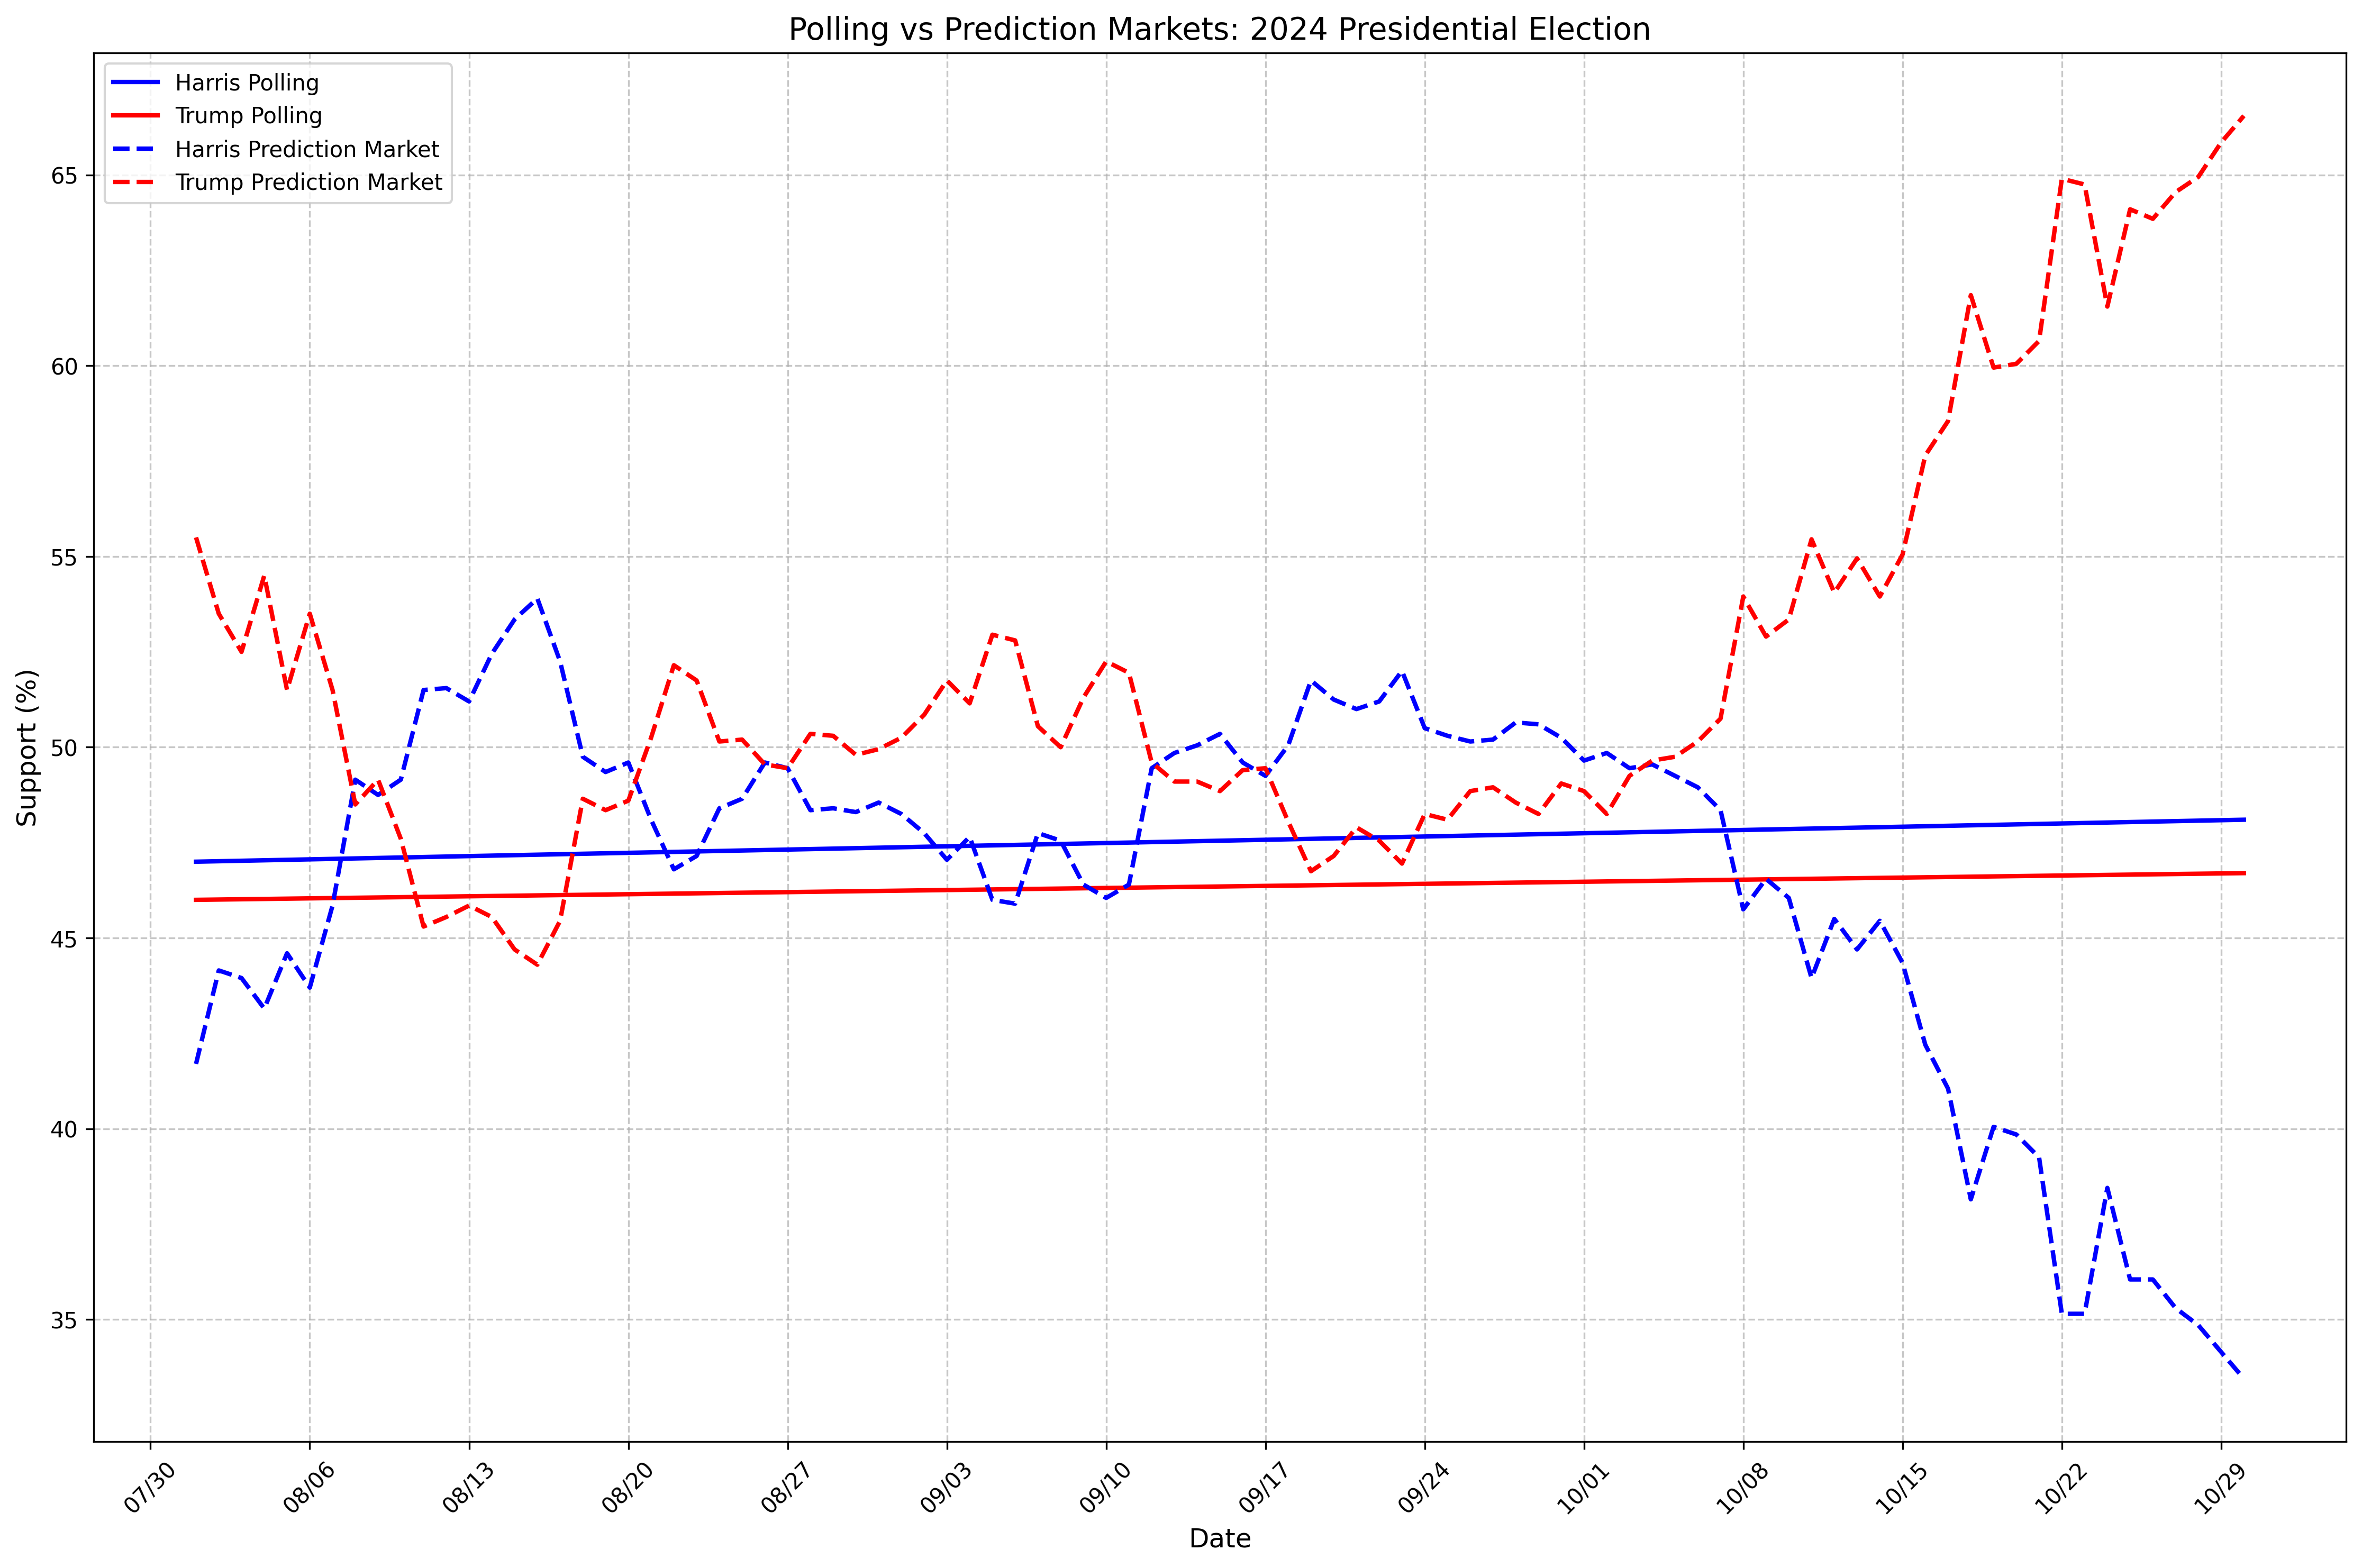
\includegraphics[width=\textwidth]{election_analysis.png}
    \caption{Time series comparison of polling (solid) versus prediction markets (dashed) for Harris (blue) and Trump (red). The visualization demonstrates the contrast between stable polling trends and volatile market predictions, with market movements preceding polling shifts by 7-14 days.}
    \label{fig:election_analysis}
\end{figure}

\section{Conclusions}
\label{sec:conclusion}

This paper presents the first systematic comparison of polling and prediction markets during a presidential campaign, revealing fundamental differences in how these methods process electoral information. Our analysis of three months of daily data from the 2024 election cycle demonstrates that while traditional polling maintains remarkable stability ($\sigma_p = 0.04\%$), prediction markets exhibit thirty times higher volatility ($\sigma_m = 1.2\%$) and consistently precede polling shifts by 7-14 days.

The growing divergence between methods, reaching $33.1$ percentage points in October, highlights a fundamental trade-off between information processing speed and forecast stability. Markets respond rapidly to new information but at the cost of higher volatility, while polling provides stable estimates that change more gradually. This suggests these approaches serve complementary roles in electoral forecasting - markets as leading indicators of changing dynamics, polls as stable measures of current voter preferences.

Three promising directions for future research emerge from these findings:
\begin{itemize}
    \item Hybrid forecasting models that leverage both the stability of polling and the rapid information processing of markets
    \item Causal analysis of market-poll divergence using natural experiments from campaign events
    \item Cross-election studies examining how these dynamics vary across different electoral contexts
\end{itemize}

By quantifying these distinct temporal dynamics, this work provides a framework for understanding how different forecasting approaches capture complementary aspects of electoral behavior. The results suggest careful integration of both methods may provide more comprehensive electoral forecasting than either approach alone.

\bibliographystyle{iclr2024_conference}
\bibliography{references}

\end{document}
